% Slides della presentazione di laurea
% Davide Tateo

\documentclass[c]{beamer}
\usepackage{lmodern}
\usepackage[utf8]{inputenc}

\usepackage{enumerate}
\usepackage{multimedia}


\usetheme{polimi}
 
\title[Cognitive SLAM]{Cognitive SLAM:}
\subtitle{Knowledge-Based Simultaneous Localization and Mapping}

\author[Davide Tateo]{Davide Tateo}
\supervisor{Relatore}{Andrea Bonarini}
\date[03/10/2014]{3 Ottobre 2014}

\begin{document}

\polimititlepage[airlab]
\addtocounter{framenumber}{-1}

%%%%%%%%%%%%%%%%%%%%%%%%%%%%%%%%%%%%%%%%%%%%%%%%%%%%%%%%%%%%%%%%%%%%%%%%%%%%%%%%%%%%%%%%%%%%%%%%%%%%%%%%%%%%%%%%%%%
\section*{Il Problema}
\begin{frame}
\frametitle{Il Problema}

Problema:
\begin{itemize}
 \item Localizzazione di robot autonomi in complessi ambienti indoor
 \item Utilizzo della conoscenza di un esperto per estrarre informazione dall'ambiente
\end{itemize}

Obiettivi:
\begin{itemize}
 \item Estrazione di feature ad alto livello (oggetti)
 \item Tracking a lungo termine degli oggetti
 \item Localizzazione basata su oggetti come landmark 
\end{itemize}

\end{frame}

%%%%%%%%%%%%%%%%%%%%%%%%%%%%%%%%%%%%%%%%%%%%%%%%%%%%%%%%%%%%%%%%%%%%%%%%%%%%%%%%%%%%%%%%%%%%%%%%%%%%%%%%%%%%%%%%%%%%

\begin{frame}
\frametitle{Sommario}
\tableofcontents
\end{frame}

%%%%%%%%%%%%%%%%%%%%%%%%%%%%%%%%%%%%%%%%%%%%%%%%%%%%%%%%%%%%%%%%%%%%%%%%%%%%%%%%%%%%%%%%%%%%%%%%%%%%%%%%%%%%%%%%%%%
\section{Stato dell'Arte}
\begin{frame}
\frametitle{Stato dell'Arte}


\begin{columns}[c, onlytextwidth]
\column{0.5\textwidth}
Sensori:
\begin{itemize}
 \item Sonar
 \item Laser
 \item Videocamere
 \item RGB-D
 \item IMU
 \item Magnetometro
 \end{itemize}

Feature:
\begin{itemize}
 \item Punti
 \item Linee
\end{itemize}

Algoritmi:
\begin{itemize}
 \item EKF-SLAM
 \item FastSLAM
\end{itemize}

\column{0.5\textwidth}

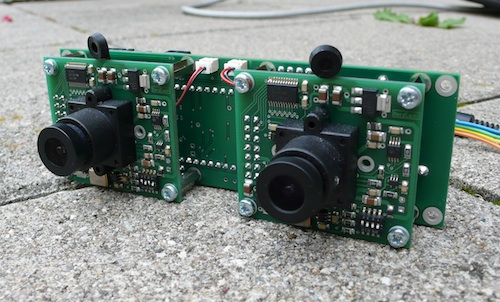
\includegraphics[width=0.9\textwidth]{immagini/stereo} \\
\vskip 0.5cm
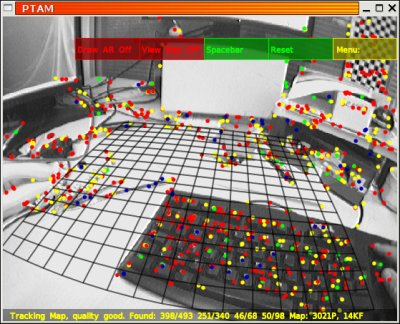
\includegraphics[width=0.9\textwidth]{immagini/ptam}


\end{columns}

\end{frame}


%%%%%%%%%%%%%%%%%%%%%%%%%%%%%%%%%%%%%%%%%%%%%%%%%%%%%%%%%%%%%%%%%%%%%%%%%%%%%%%%%%%%%%%%%%%%%%%%%%%%%%%%%%%%%%%%%%%%
\section{Struttura logica del sistema}

\begin{frame}

\frametitle{Struttura logica del sistema}

\begin{columns}[c, onlytextwidth]
 \column{.6\textwidth}
 \begin{itemize}
  \item Sistema modulare
 \begin{itemize}
  \item Reasoning
  \item Individuazione degli oggetti
  \item Riconoscimento degli oggetti
  \item Tracking
  \item Localizzazione
 \end{itemize}
  \item Utilizzo di knowledge base
  \item Tracking a lungo termine feature
  \item Approccio Full-SLAM
 \end{itemize}
 
 
 \column{.4\textwidth}
 \centering{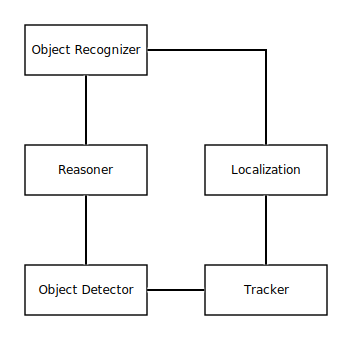
\includegraphics[width=\textwidth]{immagini/logico}}
 
 \end{columns}

\end{frame}


%%%%%%%%%%%%%%%%%%%%%%%%%%%%%%%%%%%%%%%%%%%%%%%%%%%%%%%%%%%%%%%%%%%%%%%%%%%%%%%%%%%%%%%%%%%%%%%%%%%%%%%%%%%%%%%%%%

\begin{frame}
\frametitle{Reasoning}

\begin{itemize}
\item Utilizzo della logica fuzzy per affrontare incertezze
 \begin{itemize}
  \item Incertezza sensori
  \item Incertezza modello
 \end{itemize}
\item Classificazione degli oggetti tramite classificatore fuzzy ad albero

\item Definizione di due linguaggi formali:
 \begin{itemize}
  \item Classificatore (modello oggetti)
  \item Knowledge base (symbol grounding)
 \end{itemize}

\item Algoritmo di reasoning
 \begin{itemize}
  \item Classificazione gerarchica
  \item Relazioni tra gli oggetti
 \end{itemize}
\end{itemize}



\end{frame}

%%%%%%%%%%%%%%%%%%%%%%%%%%%%%%%%%%%%%%%%%%%%%%%%%%%%%%%%%%%%%%%%%%%%%%%%%%%%%%%%%%%%%%%%%%%%%%%%%%%%%%%%%%%%%%%%%%%

\begin{frame}
\frametitle{Individuazione e riconoscimento}
\begin{itemize}
 \item Basati sulle proprietà geometriche dell'immagine
 \begin{itemize}
  \item Linee (trasformata di Hough)
  \item Cluster (DBSCAN)
  \item Rettangoli
 \end{itemize}
 \item Posa del robot per filtrare le linee orizzontali e verticali
 \item Euristiche per riconoscere i rettangoli dalle linee
 \item Classificazione delle feature tramite classificatore fuzzy ad albero
\end{itemize}

\end{frame}

%%%%%%%%%%%%%%%%%%%%%%%%%%%%%%%%%%%%%%%%%%%%%%%%%%%%%%%%%%%%%%%%%%%%%%%%%%%%%%%%%%%%%%%%%%%%%%%%%%%%%%%%%%%%%%%%%%%

\begin{frame}
\frametitle{Individuazione e riconoscimento}

\centering{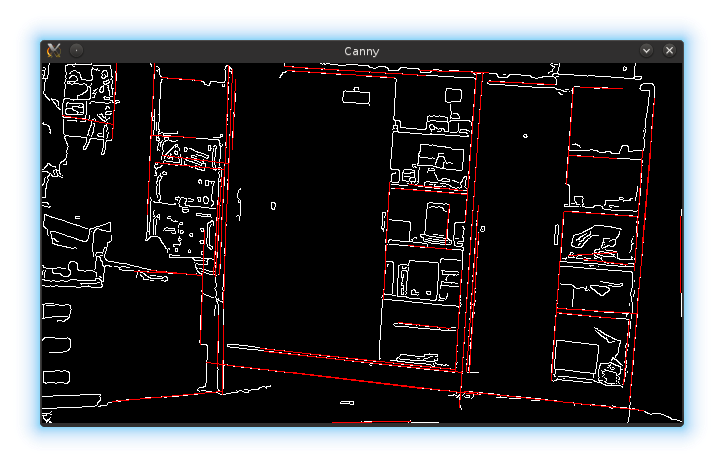
\includegraphics[width=\textwidth]{immagini/canny}} \\

\end{frame}

%%%%%%%%%%%%%%%%%%%%%%%%%%%%%%%%%%%%%%%%%%%%%%%%%%%%%%%%%%%%%%%%%%%%%%%%%%%%%%%%%%%%%%%%%%%%%%%%%%%%%%%%%%%%%%%%%%%

\begin{frame}
\frametitle{Tracking}

CMT: Consensus-based Matching and Tracking of Keypoints
\begin{columns}[c, onlytextwidth]
\column{.55\textwidth}
\begin{itemize}
 \item Algoritmo di tracking a lungo termine
 \item Basato su keypoint
 \begin{itemize}
  \item BRISK per estrarre e descrivere keypoint
  \item Optical flow per trackare i keypoint estratti
 \end{itemize}
 \item Stima di:
  \begin{itemize}
  \item scala
  \item rotazione
 \end{itemize}
 \item Clustering e politica di consenso per determinare il centro di massa

\end{itemize}
\column{.4\textwidth}
\centering{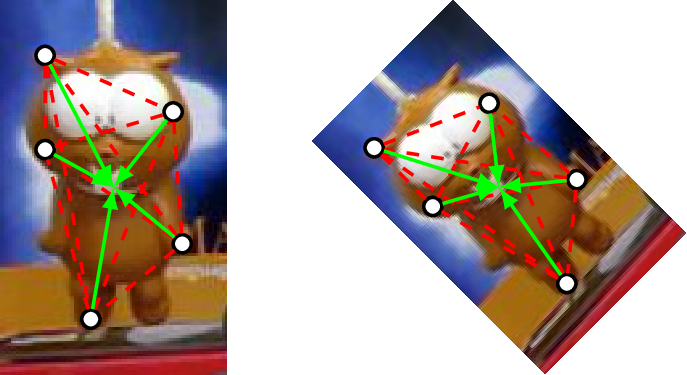
\includegraphics[width=\textwidth]{immagini/voting}} \\
\vskip 0.5cm
\centering{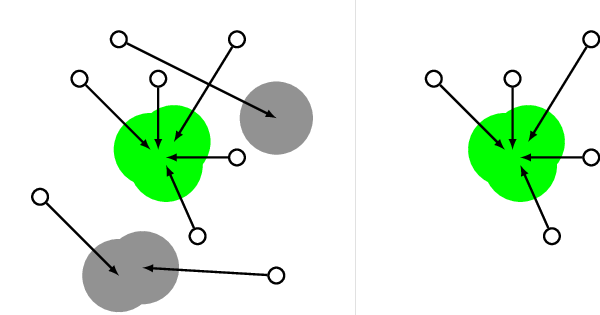
\includegraphics[width=\textwidth]{immagini/consensus}}

\end{columns}
\end{frame}

%%%%%%%%%%%%%%%%%%%%%%%%%%%%%%%%%%%%%%%%%%%%%%%%%%%%%%%%%%%%%%%%%%%%%%%%%%%%%%%%%%%%%%%%%%%%%%%%%%%%%%%%%%%%%%%%%%%

\begin{frame}
\frametitle{Mapping}

\begin{itemize}
 \item Minimizzazione dell'errore di riproiezione
 \item Stima dei landmark e pose simultanea (Approccio full-slam)
 \item Sensor fusion per integrare informazioni dagli altri sensori
 \item Stima di massima verosimiglianza su factor graph
\end{itemize}

\centering{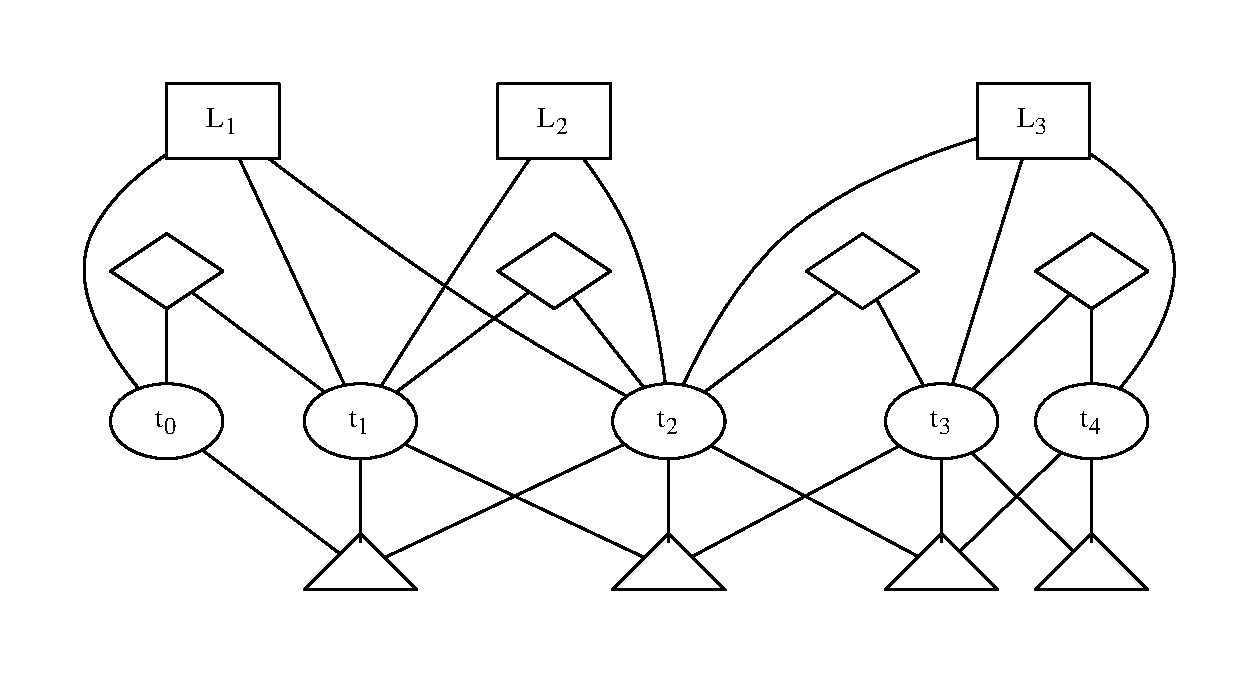
\includegraphics[width=\textwidth]{immagini/FactorGraph}}

\end{frame}

%%%%%%%%%%%%%%%%%%%%%%%%%%%%%%%%%%%%%%%%%%%%%%%%%%%%%%%%%%%%%%%%%%%%%%%%%%%%%%%%%%%%%%%%%%%%%%%%%%%%%%%%%%%%%%%%%%%

\begin{frame}
\frametitle{Mapping}

\begin{block}{Errore sulle track}
 \begin{equation*}
  \hat{L}^I =  K\cdot \left[  R^C_W \middle| t^C_W  \right] \cdot L^W
 \end{equation*}
 \begin{equation*}
  e = \hat{L}^I - L^I + \eta
 \end{equation*}
\end{block}
\vskip 1cm
\begin{block}{Errore sugli oggetti}
 \begin{equation*}
  \hat{L}^I_i =  K\cdot \left[  R^C_W \middle| t^C_W  \right] \cdot H^W_O \cdot L^O
 \end{equation*}
 \begin{equation*}
  e_i = \hat{L}^I_i - L^I_i + \eta
 \end{equation*}
\end{block}



\end{frame}


%%%%%%%%%%%%%%%%%%%%%%%%%%%%%%%%%%%%%%%%%%%%%%%%%%%%%%%%%%%%%%%%%%%%%%%%%%%%%%%%%%%%%%%%%%%%%%%%%%%%%%%%%%%%%%%%%%%

\section{Architettura del sistema}
\begin{frame}
\frametitle{Architettura del sistema}

\begin{itemize}
\item Middleware: ROS - Robot Operating System
\begin{itemize}
 \item Publish-Subscribe
 \item Client-Server
 \item Interfacce sensori
\end{itemize}

\item Fusione Multisensoriale: ROAMFREE - Robust Odometry Applying Multisensor Fusion to Reduce Estimation Errors
\begin{itemize}
 \item IMU, magnetometro
 \item Track
 \item Oggetti
\end{itemize}

\item Analisi di immagine: OpenCV 2

\item Parser del classificatore: Flex e Bison
\end{itemize}

\end{frame}

%%%%%%%%%%%%%%%%%%%%%%%%%%%%%%%%%%%%%%%%%%%%%%%%%%%%%%%%%%%%%%%%%%%%%%%%%%%%%%%%%%%%%%%%%%%%%%%%%%%%%%%%%%%%%%%%%%%

\begin{frame}
\frametitle{Architettura del sistema}

\centering{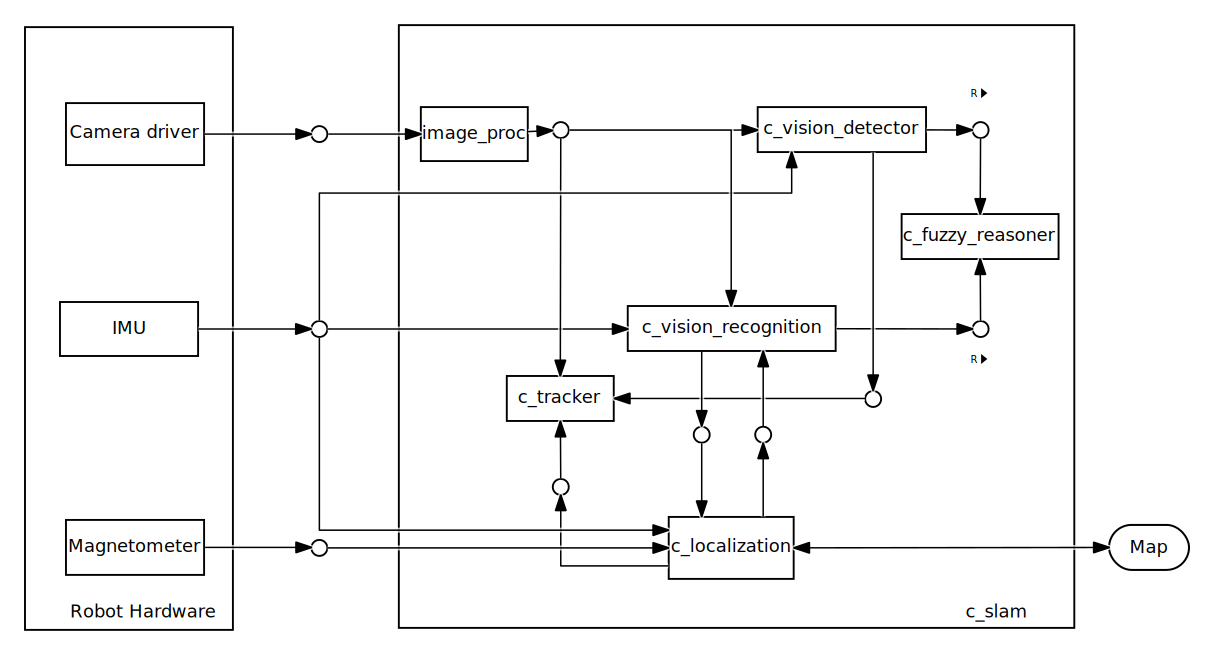
\includegraphics[width=\textwidth]{immagini/sistema}}

\end{frame}


%%%%%%%%%%%%%%%%%%%%%%%%%%%%%%%%%%%%%%%%%%%%%%%%%%%%%%%%%%%%%%%%%%%%%%%%%%%%%%%%%%%%%%%%%%%%%%%%%%%%%%%%%%%%%%%%%%%

\section{Risultati}
\begin{frame}
\frametitle{Risultati - Individuazione}
\centering{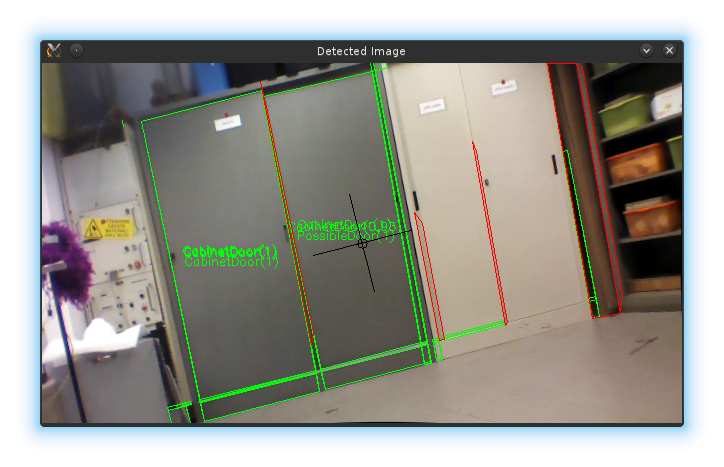
\includegraphics[width=\textwidth]{immagini/risultati/detection}}
\end{frame}

%%%%%%%%%%%%%%%%%%%%%%%%%%%%%%%%%%%%%%%%%%%%%%%%%%%%%%%%%%%%%%%%%%%%%%%%%%%%%%%%%%%%%%%%%%%%%%%%%%%%%%%%%%%%%%%%%%%

\begin{frame}
\frametitle{Risultati - Riconoscimento}
\begin{columns}[c, onlytextwidth]
 \column{0.5\textwidth}
 \centering{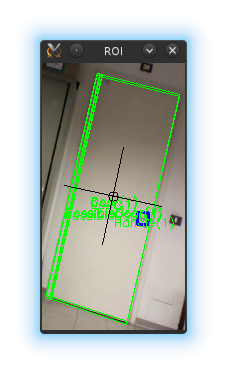
\includegraphics[width=\textwidth]{immagini/risultati/recognition1}}
 \column{0.5\textwidth}
 \centering{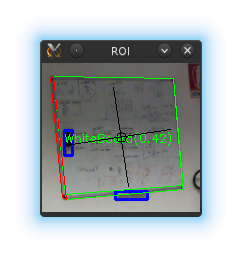
\includegraphics[width=\textwidth]{immagini/risultati/recognition2}}
\end{columns}


\end{frame}

%%%%%%%%%%%%%%%%%%%%%%%%%%%%%%%%%%%%%%%%%%%%%%%%%%%%%%%%%%%%%%%%%%%%%%%%%%%%%%%%%%%%%%%%%%%%%%%%%%%%%%%%%%%%%%%%%%%

\begin{frame}
\frametitle{Risultati - Tracking}
\centering{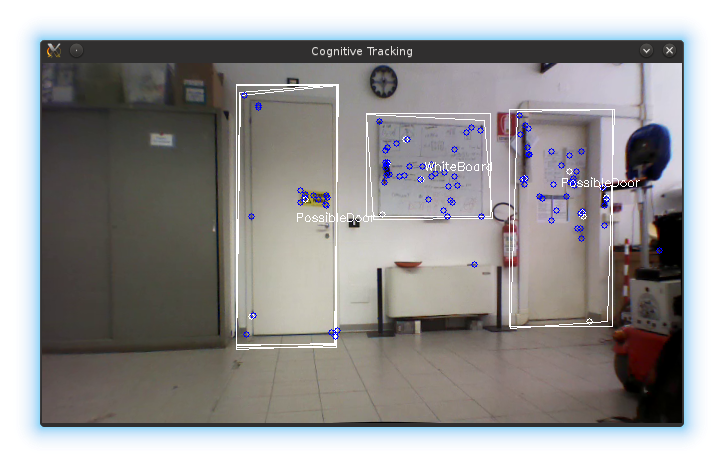
\includegraphics[height=0.45\paperheight]{immagini/risultati/tracker1}} \\
\vskip -0.5cm
\centering{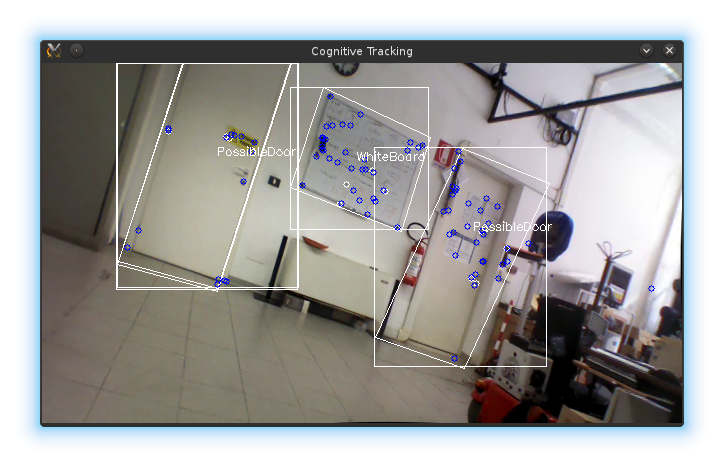
\includegraphics[height=0.45\paperheight]{immagini/risultati/tracker2}}
\end{frame}

%%%%%%%%%%%%%%%%%%%%%%%%%%%%%%%%%%%%%%%%%%%%%%%%%%%%%%%%%%%%%%%%%%%%%%%%%%%%%%%%%%%%%%%%%%%%%%%%%%%%%%%%%%%%%%%%%%%

\begin{frame}
\frametitle{Risultati - Costo computazionale}

Test effettuati su un processore i7-4500U, 4GB di ram:

\begin{itemize}
 \item individuazione e riconoscimento degli oggetti real time (in media 20/25 fps)
 \item tracking real time, frame rate medio dipendente dal numero di track seguite in parallelo (1 $\sim$20 fps, 10 $\sim$5 fps) 
 \item Mapping effettuato con tecniche batch (bundle adjustment).
 \item Localizzazione su mappa nota possibile in real time.
\end{itemize}

\end{frame}

%%%%%%%%%%%%%%%%%%%%%%%%%%%%%%%%%%%%%%%%%%%%%%%%%%%%%%%%%%%%%%%%%%%%%%%%%%%%%%%%%%%%%%%%%%%%%%%%%%%%%%%%%%%%%%%%%%%

\begin{frame}
\frametitle{Risultati - Costo computazionale}
Le prestazioni del sistema sono ampiamente migliorabili:
\begin{itemize}
 \item Algoritmi più efficienti di estrazione delle feature
 \item Feature estratte solo su keyframe
 \item Integrazione con la mappa
\end{itemize}
 
\end{frame}

%%%%%%%%%%%%%%%%%%%%%%%%%%%%%%%%%%%%%%%%%%%%%%%%%%%%%%%%%%%%%%%%%%%%%%%%%%%%%%%%%%%%%%%%%%%%%%%%%%%%%%%%%%%%%%%%%%%

\begin{frame}
\frametitle{Risultati - Video individuazione e tracking}
\movie[width=\textwidth, height = 0.8\paperheight, poster, autostart, borderwidth=1pt]{}{video/tracking.avi}
 
\end{frame}

%%%%%%%%%%%%%%%%%%%%%%%%%%%%%%%%%%%%%%%%%%%%%%%%%%%%%%%%%%%%%%%%%%%%%%%%%%%%%%%%%%%%%%%%%%%%%%%%%%%%%%%%%%%%%%%%%%%

\begin{frame}
\frametitle{Risultati - Video riconoscimento}
\begin{columns}[c, onlytextwidth]
 \column{0.5\textwidth}
 \movie[width=\textwidth, height = 0.8\paperheight, poster, autostart]{}{video/canny.avi}
 \column{0.5\textwidth}
 \movie[width=\textwidth, height = 0.8\paperheight, poster, autostart]{}{video/recognition.avi}
\end{columns}

\end{frame}

%%%%%%%%%%%%%%%%%%%%%%%%%%%%%%%%%%%%%%%%%%%%%%%%%%%%%%%%%%%%%%%%%%%%%%%%%%%%%%%%%%%%%%%%%%%%%%%%%%%%%%%%%%%%%%%%%%%

\section{Conclusioni}
\begin{frame}
\frametitle{Conclusioni}
\begin{itemize}
 \item Sistema di localizzazione basato sugli oggetti
 \item Riconoscimento degli oggetti effettuato grazie alle loro caratteristiche geometriche
 \item Mappe semantiche dell'ambiente
 \item Possibilità di fare inferenza sull'ambiente
 \item Utilizzo dell'informazione estraibile da più sensori a basso costo
 \item Sistema real-time di riconoscimento di feature
 \item Mapping con tecniche batch
\end{itemize}


\end{frame}

%%%%%%%%%%%%%%%%%%%%%%%%%%%%%%%%%%%%%%%%%%%%%%%%%%%%%%%%%%%%%%%%%%%%%%%%%%%%%%%%%%%%%%%%%%%%%%%%%%%%%%%%%%%%%%%%%%%

\begin{frame}

\vskip 0.4\paperheight

  \centering{\Huge Domande?}
  \vskip 3cm
  \begin{flushright}
     \footnotesize Powered by \fontfamily{cmr}\selectfont{\LaTeX}
  \end{flushright}
\end{frame}

\end{document}

